\FloatBarrier
\section{Experiments}
We are currently conducting experiments to replicate the results of the original papers and to evaluate the impact of various learning techniques on retrieval accuracy. We intend to conduct additional experiments in the future following the implementation of certain improvements.

\subsection{Datasets}
\begin{itemize}
    \item \textbf{FashionIQ}: At present, we are utilizing only the \textit{FashionIQ} dataset~\cite{wu2020fashioniqnewdataset}, as employed by the original study. FashionIQ is a natural language-based interactive fashion product retrieval dataset. It contains 77,684 images crawled from Amazon.com, covering three categories: Dresses, Tops \& Tees, and Shirts. Among the 46,609 training images, there are 18,000 image pairs. Each pair is accompanied by an average of two natural language sentences that describe one or multiple visual properties to modify in the reference image, such as ``is shiny'' or ``is blue in color and floral, and with white base.''
    \item \textbf{Fashion200K}: We anticipate incorporating the \textit{Fashion200K} dataset~\cite{han2017automaticspatiallyawarefashionconcept} in subsequent experiments. Fashion200K is a large-scale fashion dataset crawled from multiple online shopping websites. It contains more than 200,000 fashion images collected for attribute-based product retrieval, covering five categories: Dresses, Jackets, Pants, Skirts, and Tops. Each image is tagged with descriptive text corresponding to a product description, such as ``beige v-neck bell-sleeve top.''
    \item \textbf{Shopping100K}: We also plan to use the \textit{Shopping100K} dataset~\cite{hou2021disentanglement} in future experiments. Shopping100K is a large-scale fashion dataset of individual clothing items extracted from different e-commerce providers. It contains 101,021 images of 12 fashion attributes, covering categories such as ``collar,'' ``color,'' ``fabric,'' ``fastening,'' ``fit,'' ``gender,'' ``length,'' ``neckline,'' ``pattern,'' ``pocket,'' ``sleeve length,'' and ``sport.'' Compared to FashionIQ and Fashion200K, the Shopping100K dataset is more diverse and only contains garments in isolation.
\end{itemize}

\subsection{Evaluation Metrics}
We employed \textit{Recall@K (R@K)}~\cite{patel2022recallksurrogatelosslarge} as the primary evaluation metric, which measures the proportion of queries for which the retrieved top \(K\) images include the correct target image. \textit{Recallsubset@K (Rsubset@K)} is a similar metric, but the model retrieves images only within the semantically similar group of the reference image.

\subsection{Current Results}
We obtained results that are highly consistent with those reported in the original paper. Figure~\ref{fig:result} shows the original results.

\begin{figure*}[t]
    \centering
    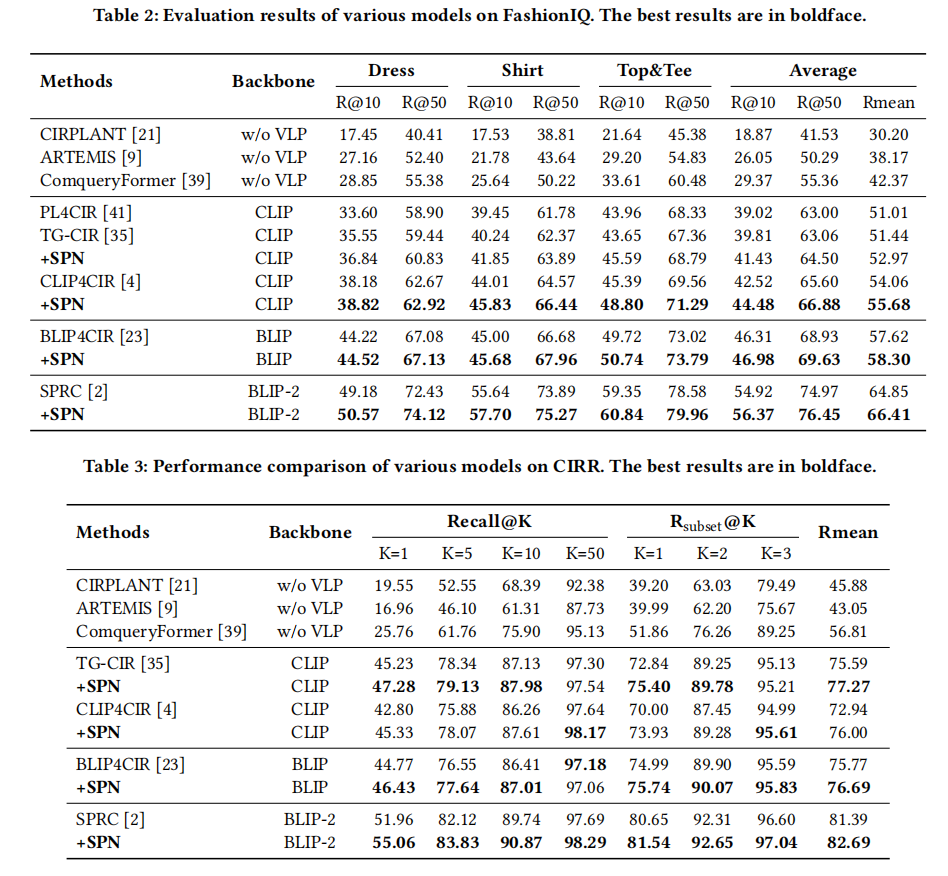
\includegraphics[width=\textwidth]{figures/result.png}
    \caption{The original paper's results.}
    \label{fig:result}
\end{figure*}

To further demonstrate the performance of our model, we present four images illustrating success and failure cases (see Figure~\ref{fig:performance}).

\begin{figure*}[t]
    \centering
    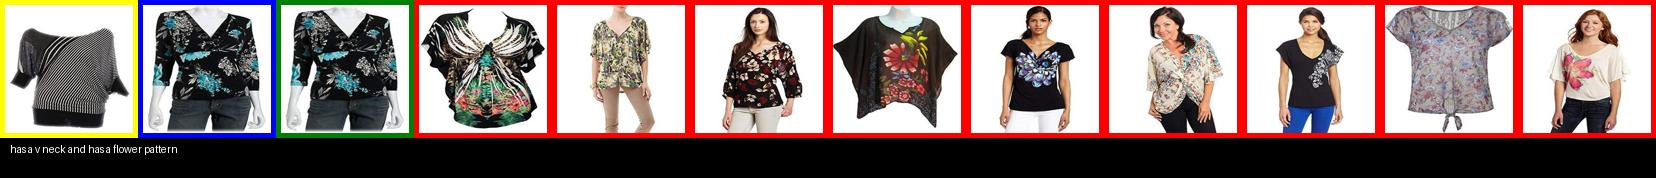
\includegraphics[width=\textwidth]{figures/success1.jpg}
    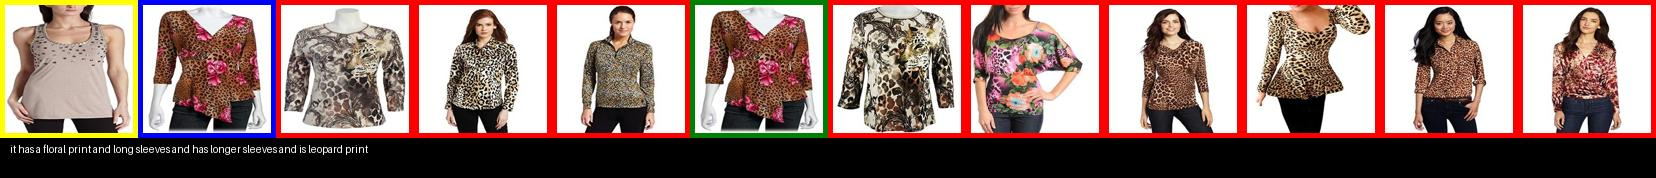
\includegraphics[width=\textwidth]{figures/success2.jpg}
    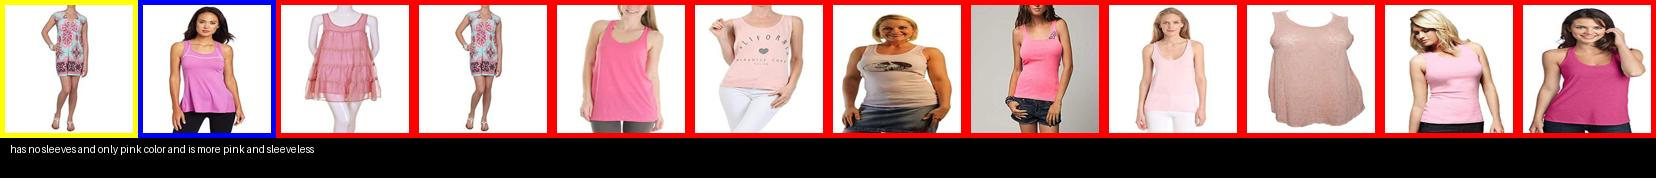
\includegraphics[width=\textwidth]{figures/failure1.jpg}
    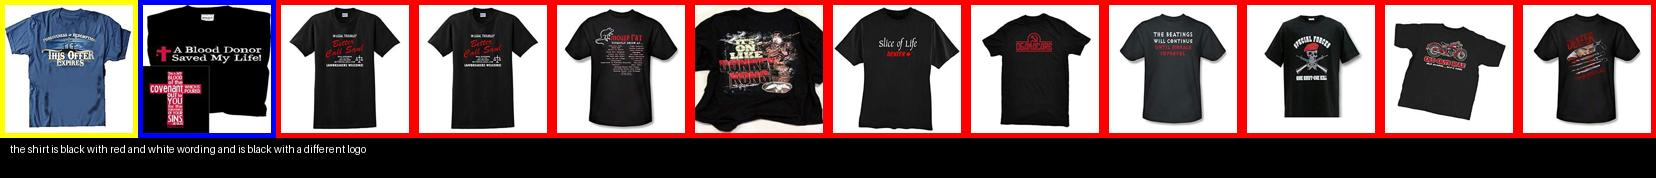
\includegraphics[width=\textwidth]{figures/failure2.jpg}
    \caption{Illustrative examples of the model's performance. The first two images represent success cases, while the last two images represent failure cases.}
    \label{fig:performance}
\end{figure*}

